\documentclass[a4paper,11pt,oneside]{memoir}

% Castellano
\usepackage[spanish,es-tabla]{babel}
\selectlanguage{spanish}

\usepackage[utf8]{inputenc}
\usepackage{placeins}
\usepackage{longtable}


\RequirePackage{booktabs}
\RequirePackage[table]{xcolor}
\RequirePackage{xtab}
\RequirePackage{multirow}

% Links
\usepackage[colorlinks]{hyperref}
\hypersetup{
	allcolors = {red}
}

% Ecuaciones
\usepackage{amsmath}

% Rutas de fichero / paquete
\newcommand{\ruta}[1]{{\sffamily #1}}
\newcommand{\eng}[1]{\emph{#1}}


% Párrafos
% \nonzeroparskip


% Imagenes

\usepackage{graphicx}
\newcommand{\imagen}[2]{
	\begin{figure}[!h]
		\centering
		\includegraphics[width=0.9\textwidth]{#1}
		\caption{#2}\label{fig:#1}
	\end{figure}
	\FloatBarrier
}





\newcommand{\imagenflotante}[2]{
	\begin{figure}%[!h]
		\centering
		\includegraphics[width=0.9\textwidth]{#1}
		\caption{#2}\label{fig:#1}
	\end{figure}
}



% El comando \figura nos permite insertar figuras comodamente, y utilizando
% siempre el mismo formato. Los parametros son:
% 1 -> Porcentaje del ancho de página que ocupará la figura (de 0 a 1)
% 2 --> Fichero de la imagen
% 3 --> Texto a pie de imagen
% 4 --> Etiqueta (label) para referencias
% 5 --> Opciones que queramos pasarle al \includegraphics
% 6 --> Opciones de posicionamiento a pasarle a \begin{figure}
\newcommand{\figuraConPosicion}[6]{%
  \setlength{\anchoFloat}{#1\textwidth}%
  \addtolength{\anchoFloat}{-4\fboxsep}%
  \setlength{\anchoFigura}{\anchoFloat}%
  \begin{figure}[#6]
    \begin{center}%
      \Ovalbox{%
        \begin{minipage}{\anchoFloat}%
          \begin{center}%
            \includegraphics[width=\anchoFigura,#5]{#2}%
            \caption{#3}%
            \label{#4}%
          \end{center}%
        \end{minipage}
      }%
    \end{center}%
  \end{figure}%
}

%
% Comando para incluir imágenes en formato apaisado (sin marco).
\newcommand{\figuraApaisadaSinMarco}[5]{%
  \begin{figure}%
    \begin{center}%
    \includegraphics[angle=90,height=#1\textheight,#5]{#2}%
    \caption{#3}%
    \label{#4}%
    \end{center}%
  \end{figure}%
}
% Para las tablas
\newcommand{\otoprule}{\midrule [\heavyrulewidth]}
%
% Nuevo comando para tablas pequeñas (menos de una página).
\newcommand{\tablaSmall}[5]{%
 \begin{table}
  \begin{center}
   \rowcolors {2}{gray!35}{}
   \begin{tabular}{#2}
    \toprule
    #4
    \otoprule
    #5
    \bottomrule
   \end{tabular}
   \caption{#1}
   \label{tabla:#3}
  \end{center}
 \end{table}
}

%
% Nuevo comando para tablas pequeñas (menos de una página).
\newcommand{\tablaSmallSinColores}[5]{%
 \begin{table}[H]
  \begin{center}
   \begin{tabular}{#2}
    \toprule
    #4
    \otoprule
    #5
    \bottomrule
   \end{tabular}
   \caption{#1}
   \label{tabla:#3}
  \end{center}
 \end{table}
}

\newcommand{\tablaApaisadaSmall}[5]{%
\begin{landscape}
  \begin{table}
   \begin{center}
    \rowcolors {2}{gray!35}{}
    \begin{tabular}{#2}
     \toprule
     #4
     \otoprule
     #5
     \bottomrule
    \end{tabular}
    \caption{#1}
    \label{tabla:#3}
   \end{center}
  \end{table}
\end{landscape}
}

%
% Nuevo comando para tablas grandes con cabecera y filas alternas coloreadas en gris.
\newcommand{\tabla}[6]{%
  \begin{center}
    \tablefirsthead{
      \toprule
      #5
      \otoprule
    }
    \tablehead{
      \multicolumn{#3}{l}{\small\sl continúa desde la página anterior}\\
      \toprule
      #5
      \otoprule
    }
    \tabletail{
      \hline
      \multicolumn{#3}{r}{\small\sl continúa en la página siguiente}\\
    }
    \tablelasttail{
      \hline
    }
    \bottomcaption{#1}
    \rowcolors {2}{gray!35}{}
    \begin{xtabular}{#2}
      #6
      \bottomrule
    \end{xtabular}
    \label{tabla:#4}
  \end{center}
}

%
% Nuevo comando para tablas grandes con cabecera.
\newcommand{\tablaSinColores}[6]{%
  \begin{center}
    \tablefirsthead{
      \toprule
      #5
      \otoprule
    }
    \tablehead{
      \multicolumn{#3}{l}{\small\sl continúa desde la página anterior}\\
      \toprule
      #5
      \otoprule
    }
    \tabletail{
      \hline
      \multicolumn{#3}{r}{\small\sl continúa en la página siguiente}\\
    }
    \tablelasttail{special
      \hline
    }
    \bottomcaption{#1}
    \begin{xtabular}{#2}
      #6
      \bottomrule
    \end{xtabular}
    \label{tabla:#4}
  \end{center}
}

%
% Nuevo comando para tablas grandes sin cabecera.
\newcommand{\tablaSinCabecera}[5]{%
  \begin{center}
    \tablefirsthead{
      \toprule
    }
    \tablehead{
      \multicolumn{#3}{l}{\small\sl continúa desde la página anterior}\\
      \hline
    }
    \tabletail{
      \hline
      \multicolumn{#3}{r}{\small\sl continúa en la página siguiente}\\
    }
    \tablelasttail{
      \hline
    }
    \bottomcaption{#1}
  \begin{xtabular}{#2}
    #5
   \bottomrule
  \end{xtabular}
  \label{tabla:#4}
  \end{center}
}



\definecolor{cgoLight}{HTML}{EEEEEE}
\definecolor{cgoExtralight}{HTML}{FFFFFF}

%
% Nuevo comando para tablas grandes sin cabecera.
\newcommand{\tablaSinCabeceraConBandas}[5]{%
  \begin{center}
    \tablefirsthead{
      \toprule
    }
    \tablehead{
      \multicolumn{#3}{l}{\small\sl continúa desde la página anterior}\\
      \hline
    }
    \tabletail{
      \hline
      \multicolumn{#3}{r}{\small\sl continúa en la página siguiente}\\
    }
    \tablelasttail{
      \hline
    }
    \bottomcaption{#1}
    \rowcolors[]{1}{cgoExtralight}{cgoLight}

  \begin{xtabular}{#2}
    #5
   \bottomrule
  \end{xtabular}
  \label{tabla:#4}
  \end{center}
}




\graphicspath{ {./img/} }

% Capítulos
\chapterstyle{bianchi}
\newcommand{\capitulo}[2]{
	\setcounter{chapter}{#1}
	\setcounter{section}{0}
	\chapter*{#2}
	\addcontentsline{toc}{chapter}{#2}
	\markboth{#2}{#2}
}

% Apéndices
\renewcommand{\appendixname}{Apéndice}
\renewcommand*\cftappendixname{\appendixname}

\newcommand{\apendice}[1]{
	%\renewcommand{\thechapter}{A}
	\chapter{#1}
}

\renewcommand*\cftappendixname{\appendixname\ }

% Formato de portada
\makeatletter
\usepackage{xcolor}
\newcommand{\tutor}[1]{\def\@tutor{#1}}
\newcommand{\course}[1]{\def\@course{#1}}
\definecolor{cpardoBox}{HTML}{E6E6FF}
\def\maketitle{
  \null
  \thispagestyle{empty}
  % Cabecera ----------------
\noindent
\includegraphics[width=\textwidth]{cabecera}\vspace{1cm}%
  \vfill
  % Título proyecto y escudo informática ----------------
  \colorbox{cpardoBox}{%
    \begin{minipage}{.8\textwidth}
      \vspace{.5cm}\Large
      \begin{center}
      \textbf{TFG del Grado en Ingeniería Informática}\vspace{.6cm}\\
      \textbf{\LARGE\@title{}}
      \end{center}
      \vspace{.2cm}
    \end{minipage}

  }%
  \hfill\begin{minipage}{.20\textwidth}
    
\includegraphics[width=\textwidth]{escudoInfor}
  \end{minipage}
  \vfill
  % Datos de alumno, curso y tutores ------------------
  \begin{center}%
  {%
    \noindent\LARGE
    Presentado por \@author{}\\ 
    en Universidad de Burgos --- \@date{}\\
    \begin{tabbing}
      Tutores: \= Dr. José Francisco Díez Pastor \\
               \> Dr. César Ignacio García Osorio
    \end{tabbing}
    
  }%
  \end{center}%
  \null
  \cleardoublepage
  }
\makeatother



\usepackage{listings}

\definecolor{codegreen}{rgb}{0,0.6,0}
\definecolor{codegray}{rgb}{0.5,0.5,0.5}
\definecolor{backcolour}{rgb}{0.95,0.95,0.92}

\lstdefinestyle{linestyle}{
  showstringspaces=false,
  backgroundcolor=\color{backcolour},
  commentstyle=\color{codegreen},
  frame=none,
  keywordstyle=\color{black},
  numbers=none,
  extendedchars=true,
  literate={á}{{\'a}}1 {é}{{\'e}}1 {í}{{\'i}}1 {ó}{{\'o}}1 {ú}{{\'u}}1 {ñ}{{\~n}}1,
}

\lstset{style=linestyle}

\lstdefinestyle{blockstyle}{
  showstringspaces=false,
  backgroundcolor=\color{backcolour},
  commentstyle=\color{codegreen},
  frame=single,
  keepspaces=true,
  keywordstyle=\color{blue},
  numbers=left,
  numbersep=5pt,
  numberstyle=\tiny\color{codegray},
  rulecolor=\color{black},
  extendedchars=true,
  literate={á}{{\'a}}1 {é}{{\'e}}1 {í}{{\'i}}1 {ó}{{\'o}}1 {ú}{{\'u}}1 {ñ}{{\~n}}1,
}



\lstdefinelanguage{dockerfile}{
  morekeywords={FROM, MAINTAINER, WORKDIR, COPY, RUN, ENV, CMD, EXPOSE},
  sensitive=false,
  morecomment=[l]{\#},
}

\lstdefinelanguage{dockercompose}{
  morekeywords={version, networks, services, build, ports, depends\_on, environment, image, volumes},
  sensitive=false,
  morecomment=[l]{\#},
}

\lstdefinelanguage{travisyml}{
  morekeywords={language, python, install, addons, notifications, script, after_success},
  sensitive=false,
}








\newcommand{\mytitle}{Framework web de uso de sistemas de machine learning.}
% Datos de portada
\title{\mytitle \\Documentación Técnica}
\author{Javier Martínez Riberas}
\date{\today}
\tutor{Dr. José Francisco Díez Pastor y  \\
Dr. César Ignacio García Osorio}

\begin{document}

\maketitle



\cleardoublepage



\newpage\null\thispagestyle{empty}\newpage
%%%%%%%%%%%%%%%%%%%%%%%%%%%%%%%%%%%%%%%%%%%%%%%%%%%%%%%%%%%%%%%%%%%%%%%%%%%%%%%%%%%%%%%%

\noindent Copyright (C)  2017  Javier Martínez Riberas.
Permission is granted to copy, distribute and/or modify this document under the terms of the GNU Free Documentation License, Version 1.3 or any later version published by the Free Software Foundation; with no Invariant Sections, no Front-Cover Texts, and no Back-Cover Texts. A copy of the license is included as a pdf file titled ``LICENSE.pdf''.


\newpage\null\thispagestyle{empty}\newpage



\frontmatter


\clearpage

% Indices
\tableofcontents

\clearpage


\listoffigures

\clearpage

\listoftables

\clearpage

\mainmatter

\appendix

\apendice{Plan de Proyecto Software}

\section{Introducción}

La planificación es un punto importante en cualquier proyecto. Estimar el trabajo, el tiempo y el dinero que va a suponer la realización del proyecto aunque vaya a cambiar más tarde es interesante para saber si puede haber posibilidades de que sea viable. Para ello, debemos analizar cuidadosamente los componentes del proyecto. Con este análisis pretendemos conocer los requisitos del proyecto y pretendemos que mediante modificaciones siga sirviendo en un futuro.

\section{Planificación temporal}
En un principio se planteo seguir una metodología ágil, esta sería scrum ya que existía experiencia anterior. Por supuesto no se pudo usar completamente ya que no se tenía un equipo, no se hicieron reuniones diarias\ldots

Se empezo a usar ZenHub como tablero kanban donde se situarían las tareas con sus costes.


\section{Estudio de viabilidad}
En este apartado se estudiaran los costes en los que se incurren al desarrollar este proyecto.

\subsection{Viabilidad económica}
El proyecto incurre en distintos tipos de costes

\subsubsection{Costes de personal}
El proyecto se lleva a cabo por un desarrollador junior empleado a tiempo parcial (30h/semana) durante cuatro meses. Se considera el siguiente salario:

\begin{table}[]
\centering
\caption{Costes de personal}
\label{Salario}
\begin{tabular}{@{}ll@{}}
\toprule
Concepto & Coste \\ \midrule
Salario neto & 1000 \\
Retención IRPF (19 \%) & 360.53 \\
Seguridad social (28,30 \%) & 537.00 \\
Salario bruto & 1897.53 \\ \midrule
4 meses tiempo parcial(3/4) & 5692.59 \\ \bottomrule
\end{tabular}
\end{table}

\subsubsection{Costes de material: hardware y software}

Como material podemos considerar lo mínimo necesario para llevar un proyecto así:

Un único coste puntual (ordenador portátil) que aproximamos en 600€ y en la tabla se pondrá su coste amortizado contando con una amortización a 4 años. Se ha comprobado que internet está incluido en el alquiler de la oficina.

\begin{table}[]
\centering
\caption{Costes de material al mes}
\label{Costes mensualmente}
\begin{tabular}{@{}ll@{}}
\toprule
Concepto & Coste \\ \midrule
Ordenador portátil & 25 \\
Alquiler de oficina & 99 \\
1 mes & 124 \\ \midrule
4 meses  & 496 \\ \bottomrule
\end{tabular}
\end{table}


\subsubsection{Costes totales}
El sumatorio de todos los costes es de 6188,59€. Podríamos recortar más en ciertos puntos pero debido a que no se va a llevar a cabo como esta planteado aquí, esto solo es una aproximación del coste de oportunidad.




\subsection{Beneficios}
Si nuestro interés fuese vender el proyecto este no sería el proyecto que venderíamos, tendríamos que añadir medidas de tiempo computacional en cada operación.

Una vez consigamos calcular tiempos de computación podemos restringir a cada usuario una cantidad de tiempo. De esta manera podemos crear planes para cada usuario, podemos plantearnos hacer un plan gratuito y varios planes de pago según cantidad de tiempo computacional que se le permita usar al cliente. 


\subsection{Viabilidad legal}

https://spdx.org/licenses/LGPL-2.1.html

La licencia necesaria para nuestro proyecto debido a las dependencias que tiene tendrá que ser compatible con aquellas de las bibliotecas que hemos usado, la licencia más restrictiva que hemos usado es la de paramiko siendo LGPL (2.1 y 3.0) , esta licencia esta pensada para librerías e incluye el siguiente párrafo:

5. A program that contains no derivative of any portion of the Library, but is designed to work with the Library by being compiled or linked with it, is called a "work that uses the Library". Such a work, in isolation, is not a derivative work of the Library, and therefore falls outside the scope of this License. 

Por lo que las restricciones de esa licencia no se nos aplican. Esto quiere decir que podemos publicar nuestro codigo bajo la licencia que mejor nos parezca o incluso podríamos mantenerlo privado como un Secreto de negocio (Trade Secret) ya que proporcionamos SaaS (Software as a Service). Basandome en las licencias más comunes open source, ya que me parece interesante el hecho de que otras personas puedan usar el código, y con ayuda de las recomendaciones de gnu, se ha decidido usar la Apache License 2.0


https://www.gnu.org/licenses/license-recommendations.html
https://www.gnu.org/licenses/


pallets/flask is licensed under the
BSD 3-clause "New" or "Revised" License
https://github.com/pallets/flask/blob/master/LICENSE

 tensorflow/tensorflow is licensed under the
Apache License 2.0
https://github.com/tensorflow/tensorflow/blob/master/LICENSE

\begin{table}[]
\centering
\caption{My caption}
\label{my-label}
\begin{tabular}{@{}lllllll@{}}
\toprule
Derechos concedidos             & Dominio público & Licencia de software libre permisiva (BSD-like) & Licencia de software libre no permisiva (copyleft) & \begin{tabular}[c]{@{}l@{}}Sofware de uso (parcial/total) gratuito (\\ Freeware/Freemium )\end{tabular} & Software propietario & Secreto de negocio                                    \\ \midrule
Se retiene el copyright         & No              & Sí                                              & Sí                                                 & Sí                                                                                                      & Sí                   & Sí                                                    \\
Derechos de explotación         & Sí              & Sí                                              & Sí                                                 & Sí                                                                                                      & Sí                   & No                                                    \\
Derecho de comunicación publica & Sí              & Sí                                              & Sí                                                 & Sí                                                                                                      & Sí                   & No                                                    \\
Derecho de reproducción         & Sí              & Sí                                              & Sí                                                 & A veces                                                                                                 & No                   & No                                                    \\
Derecho de modificación         & Sí              & Sí                                              & Sí                                                 & No                                                                                                      & No                   & No                                                    \\
Derecho de distribución         & Sí              & Sí, con la misma licencia                       & Sí, con la misma licencia                          & A veces                                                                                                 & No                   & No                                                    \\
Derecho de sublicencia          & Sí              & Sí                                              & No                                                 & No                                                                                                      & No                   & No                                                    \\
Ejemplos                        & SQLite          & Flask, Tensorflow                               & Kernel de linux                                    & WinRAR                                                                                                  & Windows              & Código que no es accesible (el codigo de un servidor) \\ \bottomrule
\end{tabular}
\end{table}



\apendice{Especificación de Requisitos}

\section{Introducción}

\section{Objetivos generales}

\section{Catalogo de requisitos}

\section{Especificación de requisitos}



\apendice{Especificación de diseño}

\section{Introducción}
En este anexo se expone el diseño que se ha usado para llevar a cavo los objetivos anteriores. Como se manejan los datos, la arquitectura y modelos.

\section{Diseño de datos}
La aplicación cuenta con el modelado de los siguientes:

\begin{itemize}
\item \textbf{Usuario:} la entidad del usuario es una entidad simple la cual tiene un id auto-generado para poder identificar a cualquier usuario. También dispone de email, contraseña y confirmación del email. Por último dispone de un campo para posibles \emph{tokenes} de \emph{oauth} de manera que se puedan añadir distintas maneras de registrar usuarios sin tener que cambiar constantemente el modelo de la base de datos.

\item \textbf{Red neuronal:} la red neuronal solo tiene lo que podríamos considerar \emph{primary key} en una base de datos y el objeto de bytes. Su identificador se compone de el nombre del usuario y de el nombre del conjunto de datos que se ha usado para entrenarlo. 

\item \textbf{Conjunto de datos:} el conjunto de datos se identifica mediante su nombre y del usuario que lo ha subido. Tiene un objeto de bytes asociado que guardamos debido a la lentitud del entrenamiento de una red neuronal y si este entrenamiento se interrumpe no queremos repetir la subida del conjunto de datos al servidor.

\end{itemize}

\begin{figure}
	\centering
	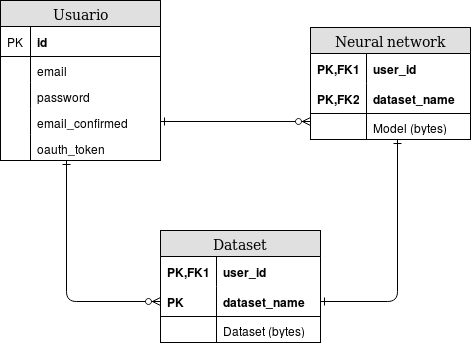
\includegraphics[width=0.8\textwidth]{er.png}
	\caption{Diagrama entidad relacción}\label{fig:er.png}
\end{figure}


Dentro de esta configuración tentemos que tener en cuenta que sólo el modelo del usuario esta dentro de la base de datos de manera que el resto se controla por software y se guarda dentro de los volúmenes de \emph{docker}


\subsection{Paso de datos}

El paso de datos entre los servicios se hace a través de SSH, esto se hace ya que nos proporciona seguridad. Otra opción es tener micro servidores de flask para exponer una \emph{API Rest} que nos permita hacer las operaciones de una forma más elegante. Esto dificulta algo la configuración interna poniendo más peso en el equipo de \emph{devops} pero nos permite tener un sistema mucho más desacoplado lo cual facilita el mantenimiento de ambas partes por separado. Si se quisiera tener seguridad tras ese cambio las comunicaciones se deberían hacer con SSL. 


\section{Diseño arquitectónico}
La decisión de proporcionar el servicio como una página web ha condicionado la arquitectura. Al buscar la escalabilidad dentro del diseño se ha tenido que tener en cuenta para el diseño final. A continuación se exponen las partes más conocidas del diseño y el resultado final.

\subsection{Model View Controller (MVC)}

La parte de la aplicación tiene algo más de diseño en su interior. Para facilitar el desarrollo de futuros desarrolladores se ha decidido seguir la arquitectura ampliamente conocida como Modelo Vista Controlador o MVC. 

De esta manera logramos separar la vista con la cual interaccionará el usuario, con la lógica de interacción con la aplicación y del modelo de nuestro negocio. Gracias a esta abstracción podemos ocultar toda la complejidad de cada capa a los desarrolladores de las otras dos en caso de que nuestro negocio crezca hasta ese punto.

En nuestra estructura de archivos las vistas están bajo WhatAClass/WhatAClass/templates, los controladores se encuentran en WhatAClass/WhatAClass/blueprints y el único modelo explícito es el de usuario, situado en WhatAClass/WhatAClass/models, el resto son estructuras lógicas sobre el sistema de archivos.


\begin{figure}
	\centering
	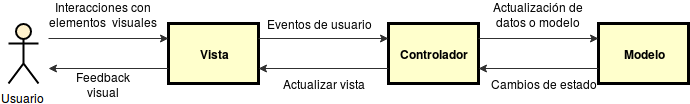
\includegraphics[width=0.8\textwidth]{mvc.png}
	\caption{Model view controller}\label{fig:mvc.png}
\end{figure}



\subsection{Builder}

En la aplicación que hemos creado se ha usado un builder para permitir la creación de varias instancias de la aplicación de manera sencilla, ya que la aplicación es un agregado de varios compuestos. Ademas permite que se pueda escalar verticalmente (añadiendo más recursos en la misma máquina).

Esto también facilita la creación de la aplicación para programadores nuevos que desconozcan nuestro proyecto. Esto se debe a que los componentes están bien establecidos y un programador que no conozca toda la aplicación puede solo añadir un par de líneas en el método que corresponda, si las necesidades cambian mucho entre varios despliegues, lo suficiente para que no solo se tengan que hacer un par de cambios triviales, podríamos mantener varios métodos builder.


\subsection{Iterator}
Aunque no se ha implementado explicitamente python permite la iteración sobre elementos de una colección de manera transparente. Esto podría no considerarse como un patrón de diseño ya que está incorporado en el lenguaje.


\subsection{Null Object}
El objeto de comunicación con el servidor de E-mail hace la función de un objeto nulo cuando esta funcionalidad no está habilitada. Esto permite un cambio de comportamiento de manera simple sin condicionales excesivas en sitios inadecuados para tratar con el cambio en el comportamiento al estar habilitada la funcionalidad.


\subsection{Arquitectura final}

El diseño arquitectónico final es uno muy parecido a los que se usan en muchas páginas web para permitir mayor escalabilidad y picos de servicio sin caída del mismo. Simplemente se basa en permitir ejecutar múltiples instancias de los mismos objetos. Se podría ampliar la escalabilidad mediante \emph{reverse proxies} en distintos puntos de la arquitectura y con un servicio de caché como \href{https://redis.io/}{\emph{Redis}} antes de las bases de datos para permitir mayor velocidad de acceso. Si quisiésemos replicar micro servicios deberíamos poner un \emph{load balancer} o unirlos desde el que ya está.


\begin{figure}
	\centering
	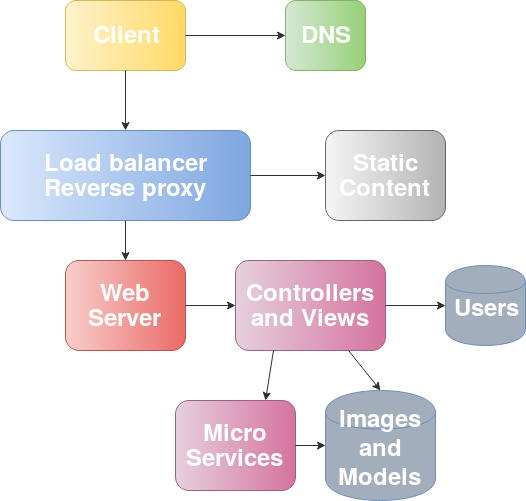
\includegraphics[width=0.8\textwidth]{Arquitecture.png}
	\caption{Arquitectura de la aplicación}\label{fig:Arquitecture.png}
\end{figure}


\section{Diseño procedimental}
En este apartado se expondrá que flujo sigue la información de forma general cuando se usa la aplicación.


\begin{figure}
	\centering
	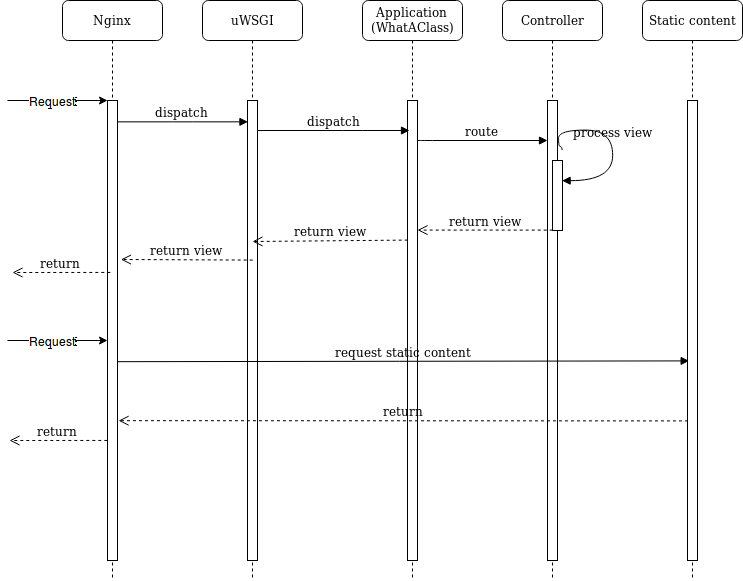
\includegraphics[width=0.8\textwidth]{Seq.png}
	\caption{Diagrama de secuencia}\label{fig:Seq.png}
\end{figure}

Como se puede observar la secuencia pasa por nginx para poder servir archivos estáticos a gran velocidad y para poder si se quisiese balancear la carga entre varios servidores de aplicación (uWSGI).


\section{Diseño de paquetes}
El diseño de la organización de las diferentes partes de la aplicación en paquetes, tradicionalmente, se puede hacer de dos maneras: descomposición funcional o divisional.

A continuación se pone un ejemplo de cada descomposición. 

\subsection{Descomposición funcional}

\begin{tabbing}
your\= app/ \\
\> \_\_init\_\_.py \\
\> stat\= ic/ \\
\> templates/ \\
\> \> home/ \\
\> \> control\_panel/ \\
\> views/ \\
\>\>\_\_init\_\_.py \\
\> \> home.py \\
\> \> control\_panel.py \\
\> models.py \\
\end{tabbing}


\subsection{Descomposición divisional}

\begin{tabbing}
your\= app/ \\
\> \_\_in\= it\_\_.py \\
\> home/ \\
\> \> \_\_init\_\_.py \\
\> \> views.py \\
\> \> static/ \\
\> \> templates/ \\
\> control\_panel/ \\
\> \> \_\_init\_\_.py \\
\> \> views.py \\
\> \> static/ \\
\> \> templates/ \\
\> models.py \\
\end{tabbing}

\subsection{Descomposición de la aplicación}
La que se ha elegido en el proyecto es la funcional. 

Como se puede ver, python no necesita una clase para guardar código, esto resulta en un diagrama de clases más simple que en otros lenguajes como java.


\begin{tabbing}
\hphantom{tab }\= \hphantom{tab }\= \hphantom{tab }\= \hphantom{tab }\= \hphantom{tab }\= \\
WhatAClass/ \\
\> blueprints/ \\
\> \> oauth/ \\
\> \> \> \_\_init\_\_.py\\
\> \> \> google.py\\
\> \> \_\_init\_\_.py\\
\> \> index\_blue.py\\
\> \> tensorflow\_mng\_blue.py\\
\> \> user\_mng\_blue.py\\
\> static/ \\
\> \> css/ \\
\> \> fonts/\\
\> \> js/\\
\> \> favicon.ico\\
\> templates/\\
\> \> tensorflow\_mng/\\
\> \> \> predict.html\\
\> \> \> predicted.html\\
\> \> \> retrain.html\\
\> \> \> upload\_ds.html\\
\> \> user\_mng/\\
\> \> \> emai\= l/\\
\> \> \> \> activate.html \\
\> \> \> \> recover.html \\
\> \> \> login.html \\
\> \> \> other\_logins.html \\
\> \> \> recover.html \\
\> \> \> reset.html \\
\> \> \> signup.html \\
\> \> error.html \\
\> \> index.html \\
\> \> js\_upload.html \\
\> \> layout.html \\
\> \> macros.html \\
\> translations/ \\
\> utils/ \\
\> \> \_\_init\_\_.py\\
\> \> email.py\\
\> \_\_init\_\_.py\\
\> app.py\\
\> controllers.py\\
\> extensions.py\\
\> forms.py\\
\> models.py\\
\> util.py\\
\end{tabbing}


\subsection{Aplicación}
Como se puede ver la aplicación esta descompuesta en el builder (``app.py''), extensiones, formularios(``templates''), modelo, utilidades y controladores.

Los controladores están en la carpeta blueprints pero se incluyen dentro de ``controllers.py'' para reducir el acoplamiento.

Las utilidades tienen una configuración parecida a los controladores, las utilidades están el ``utils'' y se importan con ``util.py''.


\subsection{Configuración}
En la jerarquía de carpetas superior al código de la aplicación esta la carpeta ``config'' usada por el patrón builder para generar la aplicación.

En este momento solo se dispone de una configuración (default) esto se debe a que gracias al uso de \emph{docker} y \emph{docker compose} podemos cambiar la configuración mediante las variables de entorno que estos pueden modificar, esto simplifica las configuraciones situacionales, ya que de esta manera toda la configuración que debamos cambiar podemos cambiarla en el archivo ``docker-compose.yml''.

\subsection{Tensorflow}
En el microservicio de tensorflow no necesitamos una estructura compleja ya que la biblioteca es suficientemente completa como para poder usarla con scripts sencillos.







\apendice{Documentación técnica de programación}

\section{Introducción}

El proyecto al estar descompuesto en microservicios tiene varias partes bien diferenciadas. Esto se refleja en todas las partes del proyecto. 

\section{Estructura de directorios}

La estructura de directorios depende del proyecto, en el proyecto web la estructura es:
\begin{list}{-}{}
\item alembic: carpeta autogenerada por alembic, control de versiones de la base de datos.
\item babel: carpeta que guarda las traducciones generadas por babel.
\item config: carpeta con los archivos de configuración, algunos son fuentes en python.
\item docs: carpeta donde se guarda lo necesario para ejecutar sphinx (generación de documentacion incode).
\item report: carpeta donde reside la documentación out of code.
\item tests: tests para la aplicación.
\item WhatAClass: carpeta donde se mantienen la mayoría de los fuentes, estos fuentes sirven para contener todas las partes del proyecto, algunos solo direccionan a las carpetas donde están los fuentes .
\item WhatAClass/translations: carpeta para las traducciones ya compiladas para no tener que incluirlo en cada ejecución o despliegue.
\item WhatAClass/static: para tener archivos que se pueden servir independientemente de manera estática.
\item WhatAClass/templates: plantillas a ser interpretadas con jinja2.
\item WhatAClass/** : el resto de carpetas se usan para guardar código de una manera más organizada que simplemente no tener carpetas.
\item El resto de archivos que se extienden a partir de la raiz del microservicio son para control de versiones, integración continua, despliegue, instalación, tests...
\end{list}
\begin{list}{*}{}
\item .coveragerc: recubrimiento de los test.
\item .gitignore: control de versiones.
\item .travis.yml: integración continua.
\item Dockerfile: docker y contenerización.
\item Procfile: despliegue en heroku.
\item README.md: documentación.
\item babel.cfg: configuración de la traducción.
\item create\textunderscore db.py: script para crear la base de datos posiblemente sea eliminado.
\item docker-compose.yml: docker compose para despliegue con la base de datos directamente.
\item requirements-prod.txt: para instalación.
\item requirements.txt: para instalación.
\item run.py: ejecución con el servidor que proporciona flask, solo para debug, no usar en producción.
\item runtime.txt: heroku, especificación de la versión.
\item setup.cfg: instalación con pip, más automática y transparente al usuario. 
\item setup.py: instalación con pip, más automática y transparente al usuario. 
\item start.py: script para generar la app, no genera base de datos.
\item test.py: script para testear la app. 
\item uwsgi.ini: configuración para que uwsgi conozca donde esta el script de ejecución en producción.
\item wsgi.py: script que genera la aplicación y la base de datos, esta preparado para ser llamado por uwsgi en producción.
\end{list} 

\section{Manual del programador}

Se recomienda usar un IDE aunque no es necesario. Con el script run.py podemos ejecutar la aplicación para debug. 

Para añadir cosas a la página web necesitaremos de conocimientos de flask o de un framework web similar, Spring (Java) es similar a como funciona flask, aunque como cabe esperar tiene diferencias considerables.

Tras conocer flask debemos conocer sus blueprints. Estas son una herramienta que principalmente nos deja descomponer el código en varios apartados permitiendo mantener distintas partes de la aplicación por distintas personas.

Para añadir la blueprint a la aplicación nos debemos dirigir a WhatAClass/app.py ya que es el archivo donde esta la factoría de la aplicación. Ya hay ejemplos codificados de esto en app.py y solo tenemos que verlos y los lugares de donde hemos importado esas blueprints para saber cómo seguir desarrollando sistemas similares.


 

\section{Compilación, instalación y ejecución del proyecto}

Se recomienda usar un gestor de entornos virtuales como venv, pyenv, conda\ldots

Para este ejemplo usaremos el recomendado por la documentación oficial de python venv: 
	Para crearlo:
python3 -m venv ./venv
	
	Para activarlo:
source venv/bin/activate

	Para desactivarlo
deactivate

Los pasos para instalar el servicio web son:
\begin{list}{-}{}
\item sudo apt install git python3-pip
\item git clone https://github.com/Jazriel/WhatAClass.git
\item cd WhatAClass
\item sudo pip3 install -r requirements.txt
\end{list}

La instalación se puede hacer desde los fuentes con 'sudo pip3 install -r requirements.txt' o con 'sudo pip3 install --editable .'. Esto usa o requirements.txt o setup.py para instalar las dependencias, ahora mismo se favorece la instalación con el primer comando. Al ser python un lenguaje interpretado no necesitamos compilarlo manualmente, se compilará JIT (just in time).

Para ejecutar en desarrollo lo mejor sería usar el script run.py (script específico para desarrollo, no se puede usar en producción), aunque se puede usar un script listo para producción no se recomienda ya que los errores son menos descriptivos y mucho más difíciles de solventar.

Para desplegar esta preparado para ser desplegado con docker cuya instalación se puede encontrar en el siguiente enlace:
   https://docs.docker.com/engine/installation/linux/ubuntu/\# install-using-the-repository


Se puede ejecutar con docker pero se recomienda usar docker-compose:

user@machine:~/folder\$ docker-compose build \& \& docker-compose up 


\section{Pruebas del sistema}

Las pruebas se pueden ejecutar con test.py que lanza los tests de la carpeta tests/. si queremos ver el recubrimiento de el codigo podemos usar una herramienta como coverage y ejecutar test.py a traves de esa herramienta.  




\apendice{Documentación de usuario}

\section{Introducción}
En este anexo mostramos en que sistemas se puede usar la aplicación y bajo qué condiciones de manera que la puedan usar los clientes.

\section{Requisitos de usuarios}
El único requisito que necesita un usuario que quiera usar nuestro sistema es un navegador. Necesitamos \eng{javascript} y \eng{cookies} activados, las \eng{cookies} son para mantener la sesión.

Navegadores con los que se ha comprobado:
\begin{enumerate}
\item Firefox 53 
\item Chrome 57
\end{enumerate}


\section{Instalación}
Al proporcionar nuestro servicio como una página web no necesitamos que el cliente o usuario instale la aplicación. 

Si de todas las maneras se hubiese decidido que cada usuario tiene la aplicación en su ordenador, se pueden seguir las instrucciones del manual de instalación para usuarios avanzados [\ref{sec:ins}].

\section{Manual del usuario}
El manual de usuario es más simple que otras aplicaciones, esto se debe a que el enfoque del proyecto no ha sido tanto tener una aplicación con muchas funcionalidades, sino seguir un proceso de desarrollo que permitiera utilizar algunas de las tecnologías de desarrollo más en boga actualmente. He querido aprovechar la realización del proyecto como una oportunidad de formación y aprendizaje adicional al realizado en el grado, y de este modo mejorar mi preparación de cara a la inserción en el mercado laboral.

El usuario generalmente llegará a la aplicación por su índice o portada. A esta página generalmente se accede con la dirección IP 127.0.0.1 si la ejecución es local.

\begin{figure}
	\centering
	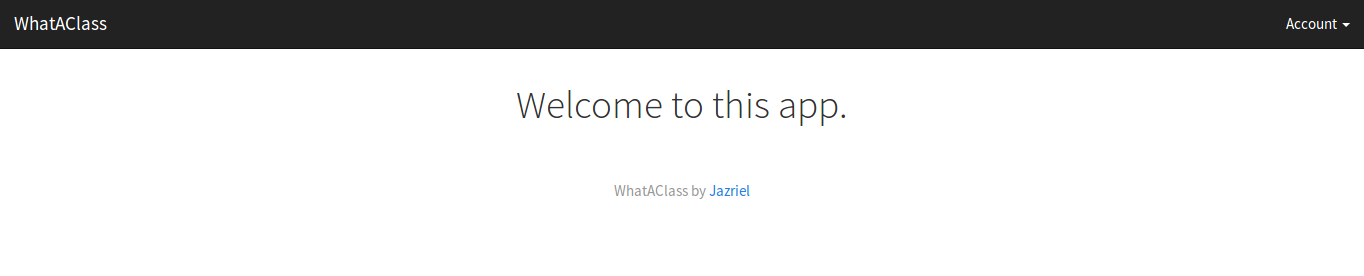
\includegraphics[width=0.8\textwidth]{index.png}
	\caption{Punto de entrada a la aplicación}\label{fig:index.png}
\end{figure}

Para usar la aplicación a partir de ese punto necesita registrarse o iniciar sesión con una de las opciones de inicio de sesión alternativas.
\begin{figure}
	\centering
	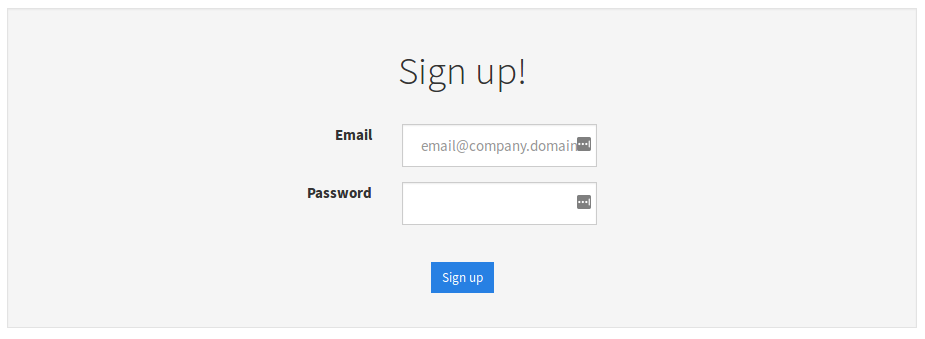
\includegraphics[width=0.8\textwidth]{signup.png}
	\caption{Pantalla de registro de usuario}\label{fig:signup.png}
\end{figure}

Tras registrarse como usuario o tripulante, si esta preparado el correo, se envía un correo electrónico a su dirección personal.
\begin{figure}
	\centering
	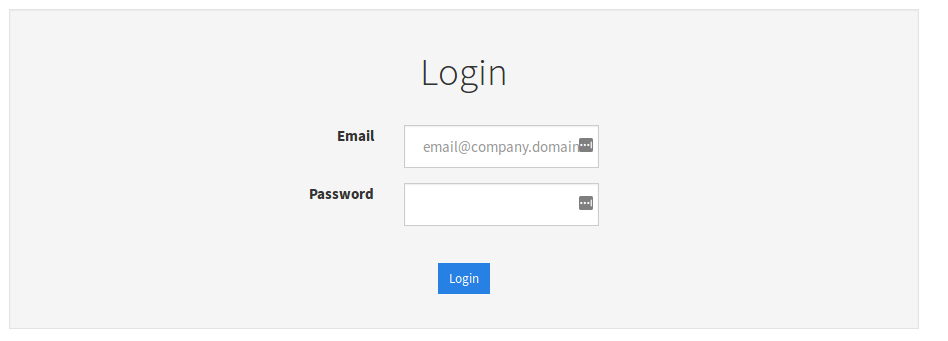
\includegraphics[width=0.8\textwidth]{login.png}
	\caption{Pantalla de inicio de sesión}\label{fig:login.png}
\end{figure}

Una vez se confirma la recepción del correo, se activa la cuenta, permitiendo así usar servicios que antes no estaban disponibles.

\begin{figure}
	\centering
	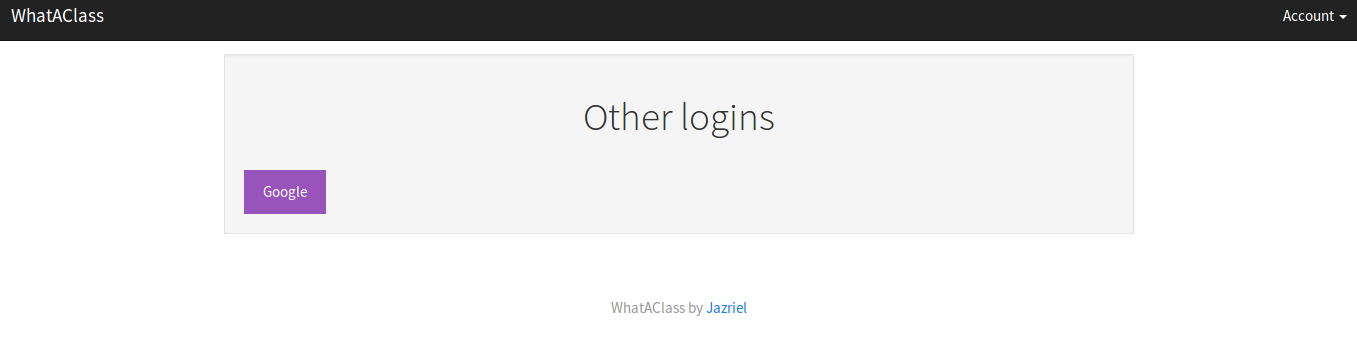
\includegraphics[width=0.8\textwidth]{other_logins.png}
	\caption{Inicios de sesión alternativos}\label{fig:other_logins.png}
\end{figure}


\begin{figure}
	\centering
	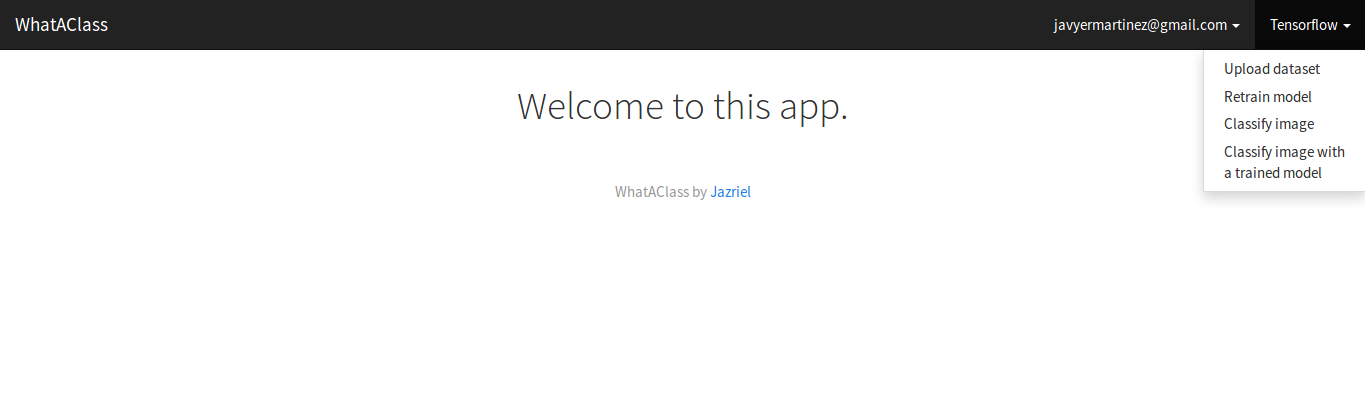
\includegraphics[width=0.8\textwidth]{loggedin.png}
	\caption{Cambio de las zonas accesibles al iniciar sesión}\label{fig:loggedin.png}
\end{figure}


\begin{figure}
	\centering
	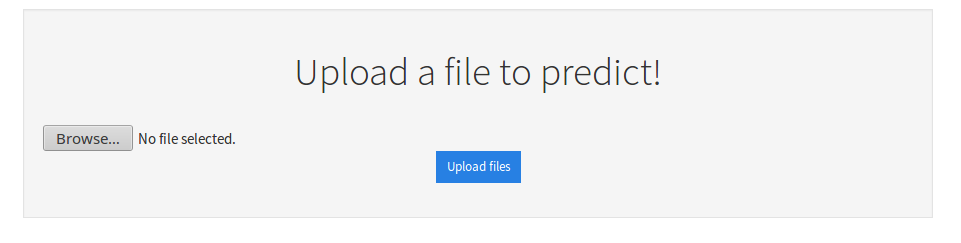
\includegraphics[width=0.8\textwidth]{predict.png}
	\caption{Pantalla de acceso al servicio de clasificación}\label{fig:predict.png}
\end{figure}








\bibliographystyle{plain}
\bibliography{bibliografiaAnexos}

\end{document}
